\documentclass[12pt,a4paper]{article}

\usepackage[dvipdfm,final]{graphics,graphicx} % dvips graphics driver
\author{Peter R.T. Munro}
\title{Matlab and C array conversion}
\begin{document}
\maketitle
This theory could be developed for a multidimensional array however I
will restrict it to arrays of tow and threee dimensions. Matlab
constructs its arrays by laying them out row-wise in memory. This is
depicted below in Figure 
\begin{figure}[h]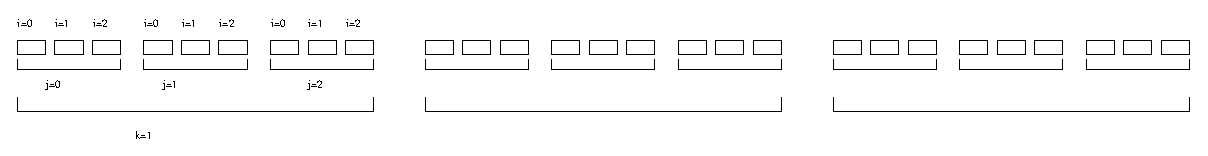
\includegraphics[width=1.\textwidth]{array.eps}
%\begin{figure}[h]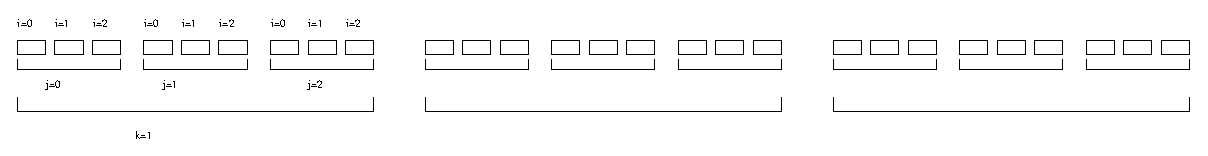
\includegraphics{array.eps}
\caption{Layout of a matlab array in memory}
\label{fig:matlab:array}
\end{figure}

This depicts an $3\times3\times3$ array that would be index according
to:

\begin{verbatim} 
>> array(i,j,k) 
\end{verbatim}
in matlab. Then the array could be pictured as being composed of rows
indexed by $i$, columns indexed by $j$ and layers indexed by $k$. The
address of a particular element \verb1array(i,j,k)1 in memory is thus given by:

\begin{verbatim} 
(mArray +k*nrows*ncols+ j*nrows + i)
\end{verbatim}

where \verb1mArray1 is the \verb1(double *)1 pointer given within the
\verb1mexFunction1. Thus the array can be indexed this way. It is also
possible to cast the memory in such a way that it can be indexed using
the usual array notation \verb1array[k][j][i]1 where one should note
that the indices are in reverse order.

In order to do this we must declare a variable of type
\verb1(double ***)1. It is structed so that if \verb1array1 is our
pointer, then \verb1array[k]1 points to a layer (see diagram). Then
\verb1array[k][j]1 points to a column within a layer. The the final
index is \verb1i1 which is used to traverse along the row. The code
for performing this is included below.

\begin{verbatim}
/*Casts a 3-dimensional array such that it may be indexed according to the 
  usual array indexing scheme array[k,j,i].

  array is a point to a matlab 3 dimensional array
  nrows the number of rows in the array
  ncols the number of columns in the array
  nlayers the number of layers, each of dimension nrows*ncols 

*/

double ***castMatlab3DArray(double *array, int nrows, int ncols, int nlayers){
  double ***p;
  int i,j,k;

  p = (double ***)malloc((unsigned) (nlayers*sizeof(double **)));
  for(k =0; k<nlayers;k++)
    p[k] = (double **)malloc((unsigned) (ncols*sizeof(double *)));
  
  for(k =0; k<nlayers;k++)
    for(j =0; j<ncols;j++)
      p[k][j] = (array + k*nrows*ncols+ j*nrows);
  return p;

}

/*Frees the axilliary memory used by the castMatlab3DArray
 */
void freeCastMatlab3DArray(double ***castArray, int nlayers){
  for(int k =0; k<nlayers;k++)
    free(castArray[k]);
  free(castArray);
}
\end{verbatim}

\end{document}
